\chapter{\texorpdfstring{Conformance Checking}{Conformance Checking}}
\label{ch:19}
\lecturemeta{Lezione 19 \quad\textbullet\quad 2026-07-04 \quad\textbullet\quad Roberto Bruni}{van der Aalst, \emph{Process Mining}, Ch.1, 6}

Con il \hyperref[ch:05]{process mining} avevamo visto come \textbf{scoprire} un modello a partire da un event log (l'α-algorithm). Questa lezione affronta la domanda complementare: dato un modello (magari scoperto, magari disegnato a mano) e un log \textbf{reale}, \textbf{quanto bene il modello descrive ciò che è realmente accaduto}? È il problema della \textbf{conformance checking}.

\begin{boxabstract}{Il quadro}
Si confrontano due fonti indipendenti di informazione: il \textbf{modello} (comportamento \emph{previsto}) e il \textbf{log} (comportamento \emph{osservato}). Il confronto produce due tipi di risultato: \textbf{misure globali} (un numero che quantifica quanto il modello e il log si somigliano) e \textbf{diagnostica locale} (dove esattamente, nel modello, log e realtà divergono).
\end{boxabstract}

\begin{figure}[!htb]
\centering
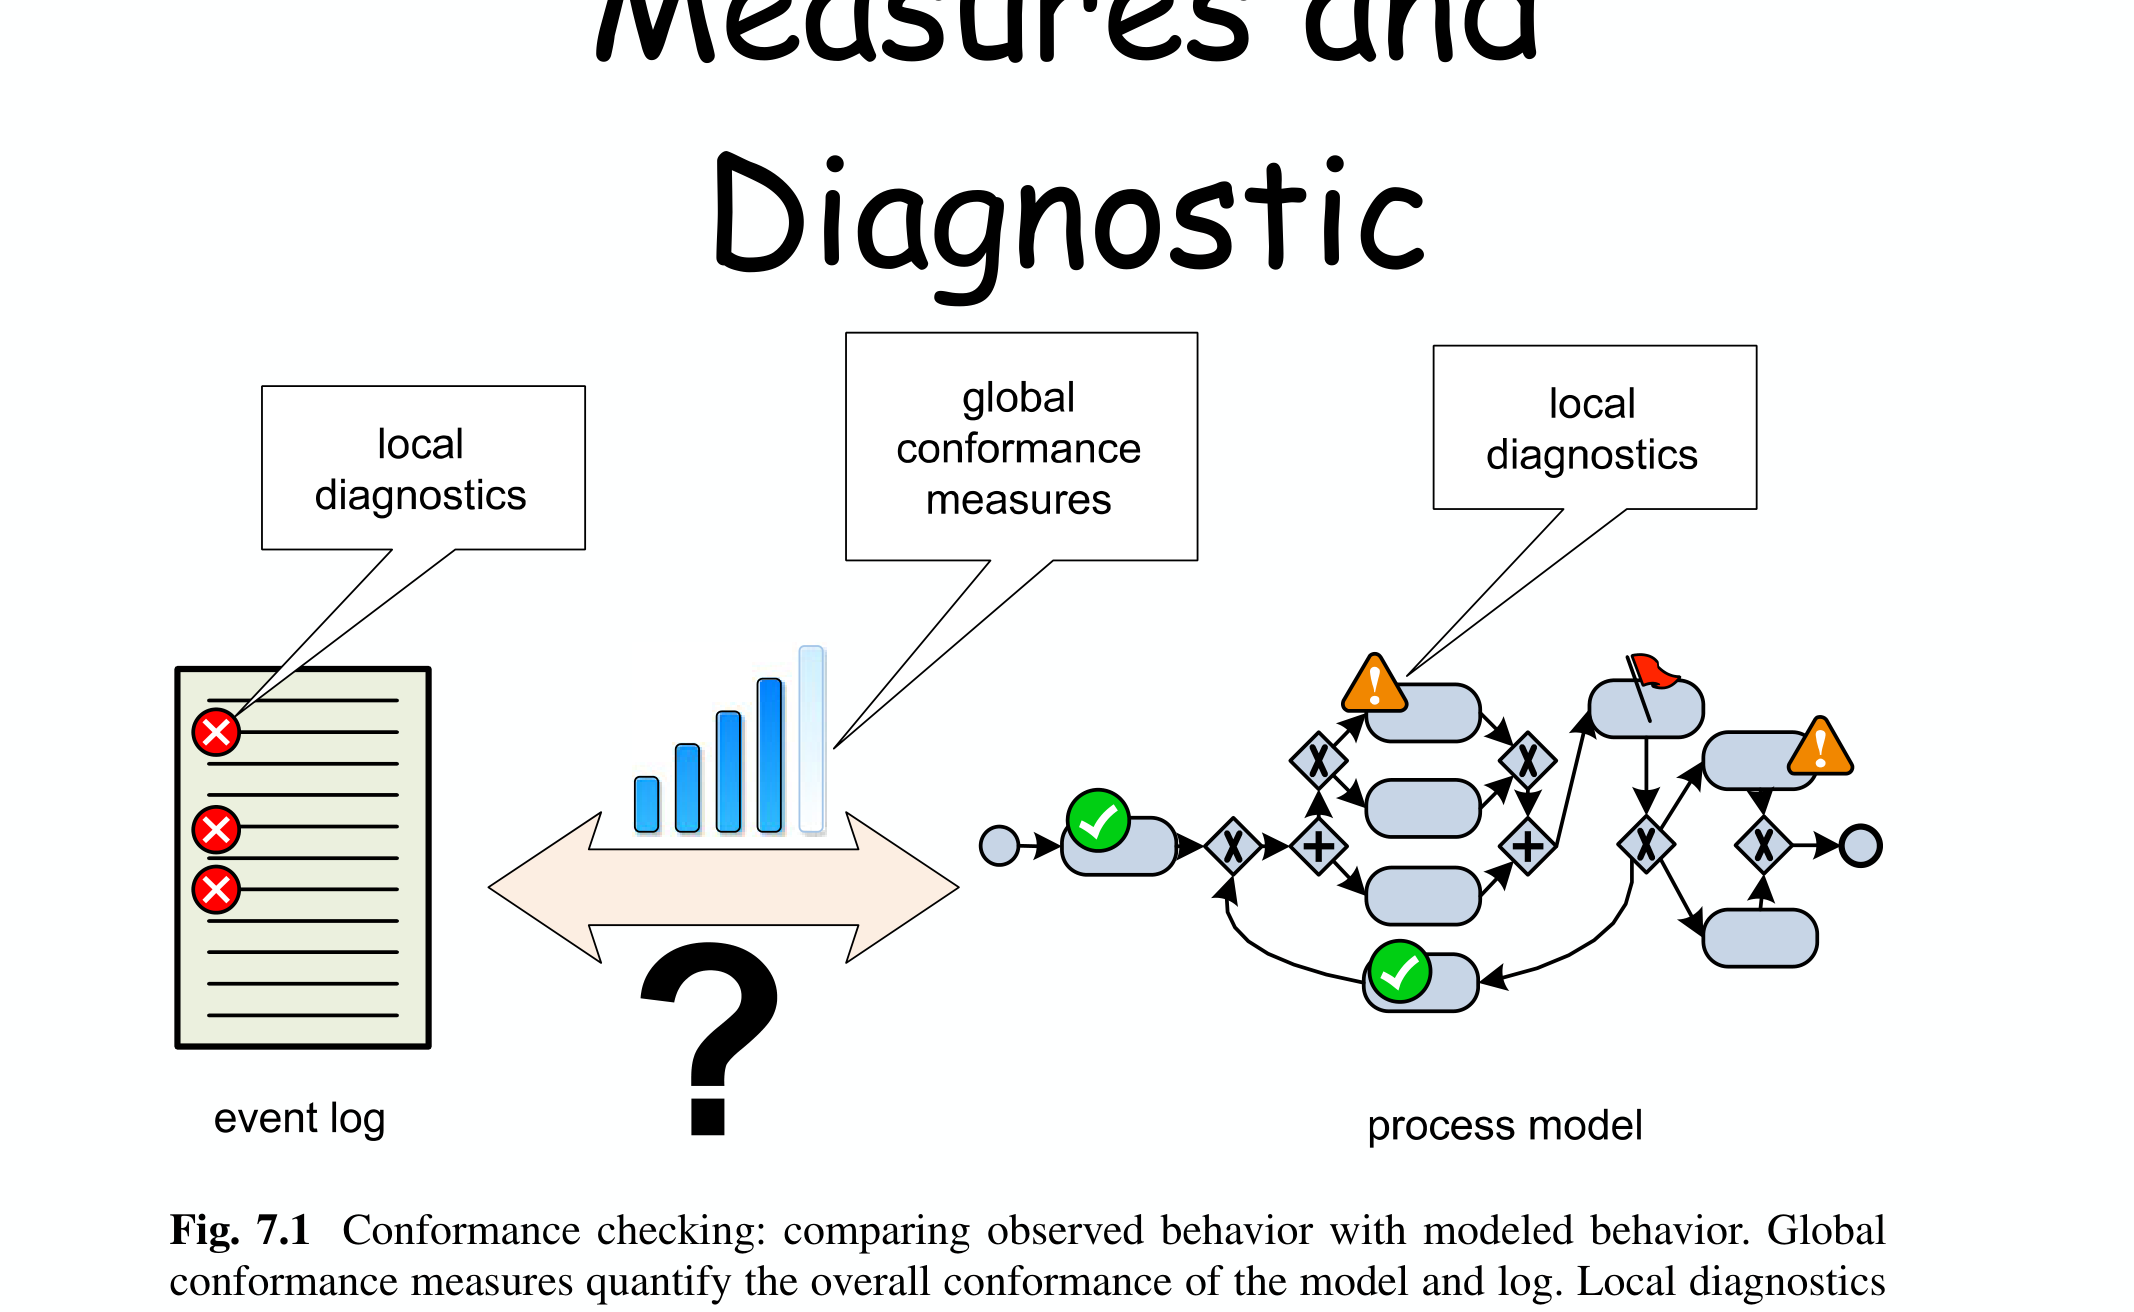
\includegraphics[width=0.74\linewidth,height=0.34\textheight,keepaspectratio]{images/19-conformance_p4_measures-diagnostic.png}
\caption{Conformance checking: si confronta il comportamento \emph{osservato} (log) con quello \emph{modellato}. Le \textbf{misure globali} riassumono in un numero quanto i due concordano; la \textbf{diagnostica locale} indica \emph{dove} nel modello (o quali casi nel log) causano il disaccordo.}
\end{figure}

\section{\texorpdfstring{Un primo tentativo: la fitness ingenua}{Un primo tentativo: la fitness ingenua}}

La \textbf{fitness} misura "la proporzione di comportamento nel log ammessa dal modello" — fra i vari criteri di qualità di un modello (fitness, precision, generalization, simplicity), è quella più vicina all'idea intuitiva di conformance.

Il modo più ovvio per calcolarla: contare quante \textbf{trace} del log corrispondono a una \textbf{firing sequence} completa del net (dal place iniziale a quello finale).

\begin{boxdefinition}{Ability to replay}
Chiedersi se il net $N$ può \textbf{"riprodurre" (replay)} una trace $\sigma$ equivale a chiedere se $\sigma \in L(N)$, il \hyperref[ch:12]{linguaggio del net}. Se $\sigma \notin L(N)$, diciamo che $\sigma$ è \textbf{non-fitting} per $N$.

\textbf{Fitness ingenua}: la frazione di casi del log la cui trace sta in $L(N)$.
\end{boxdefinition}

Il problema di questa metrica "tutto o niente" emerge subito su un esempio concreto: un log con 1391 casi confrontato con quattro modelli diversi ($N_1$, $N_2$, $N_3$, $N_4$) dà fitness ingenue molto diverse — $1$, $0.68$, $0.45$, $1$ — ma i due modelli con fitness $1$ sono agli antipodi: uno è un modello sensato che effettivamente cattura tutto il comportamento osservato, l'altro è un \textbf{flower model} (un modello degenerato, permissivo al punto da accettare qualsiasi sequenza, e quindi banalmente "conforme" a tutto — ma inutile).

\begin{boxwarning}{Il difetto della fitness ingenua}
Una trace che il modello non riesce a riprodurre viene scartata \textbf{appena si trova il primo problema}, senza distinguere fra "quasi conforme" (manca un solo evento su cento) e "completamente diversa" (ne mancano novanta). Entrambe finiscono etichettate allo stesso modo: \textbf{non-fitting}. Serve una misura più \textbf{granulare}.
\end{boxwarning}

\section{\texorpdfstring{Token replay: contare i token mancanti e residui}{Token replay: contare i token mancanti e residui}}

L'idea per raffinare la misura: invece di fermarsi al primo problema, si \textbf{continua} a "riprodurre" la trace sul net \textbf{forzando} le transizioni a scattare anche quando non sono abilitate, e si \textbf{contano gli errori} invece di limitarsi a segnalarli.

\begin{boxdefinition}{I quattro contatori del token replay}
Per ogni trace $\sigma$ riprodotta su un net $N$ si tengono quattro contatori: - $p$ — token \textbf{prodotti} in totale durante la riproduzione; - $c$ — token \textbf{consumati} in totale; - $m$ — token \textbf{mancanti} (\emph{missing}): ogni volta che una transizione deve scattare ma un place di input non ha il token, si registra il "buco" e si forza comunque lo scatto; - $r$ — token \textbf{residui} (\emph{remaining}): quelli che restano nella rete alla fine, invece di essere consumati dall'ambiente al termine del caso.
\end{boxdefinition}

\begin{boxtheorem}{Formula della fitness}
\[
\text{fitness}(\sigma, N) = \frac{1}{2}\left(1 - \frac{m}{c}\right) + \frac{1}{2}\left(1 - \frac{r}{p}\right)
\]

Le due metà sono \textbf{pesate ugualmente} e misurano due difetti distinti:

\[
\frac{m}{c} = \text{proporzione di consumi "forzati" (mancava il token)}
\]

\[
\frac{r}{p} = \text{proporzione di produzioni "sprecate" (token che restano inutilizzati)}
\]

Il caso \textbf{ideale} è $m = r = 0$, che dà fitness $= 1$.
\end{boxtheorem}

\subsection{\texorpdfstring{Esempio: nessun token mancante né residuo}{Esempio: nessun token mancante né residuo}}

\begin{figure}[!htb]
\centering
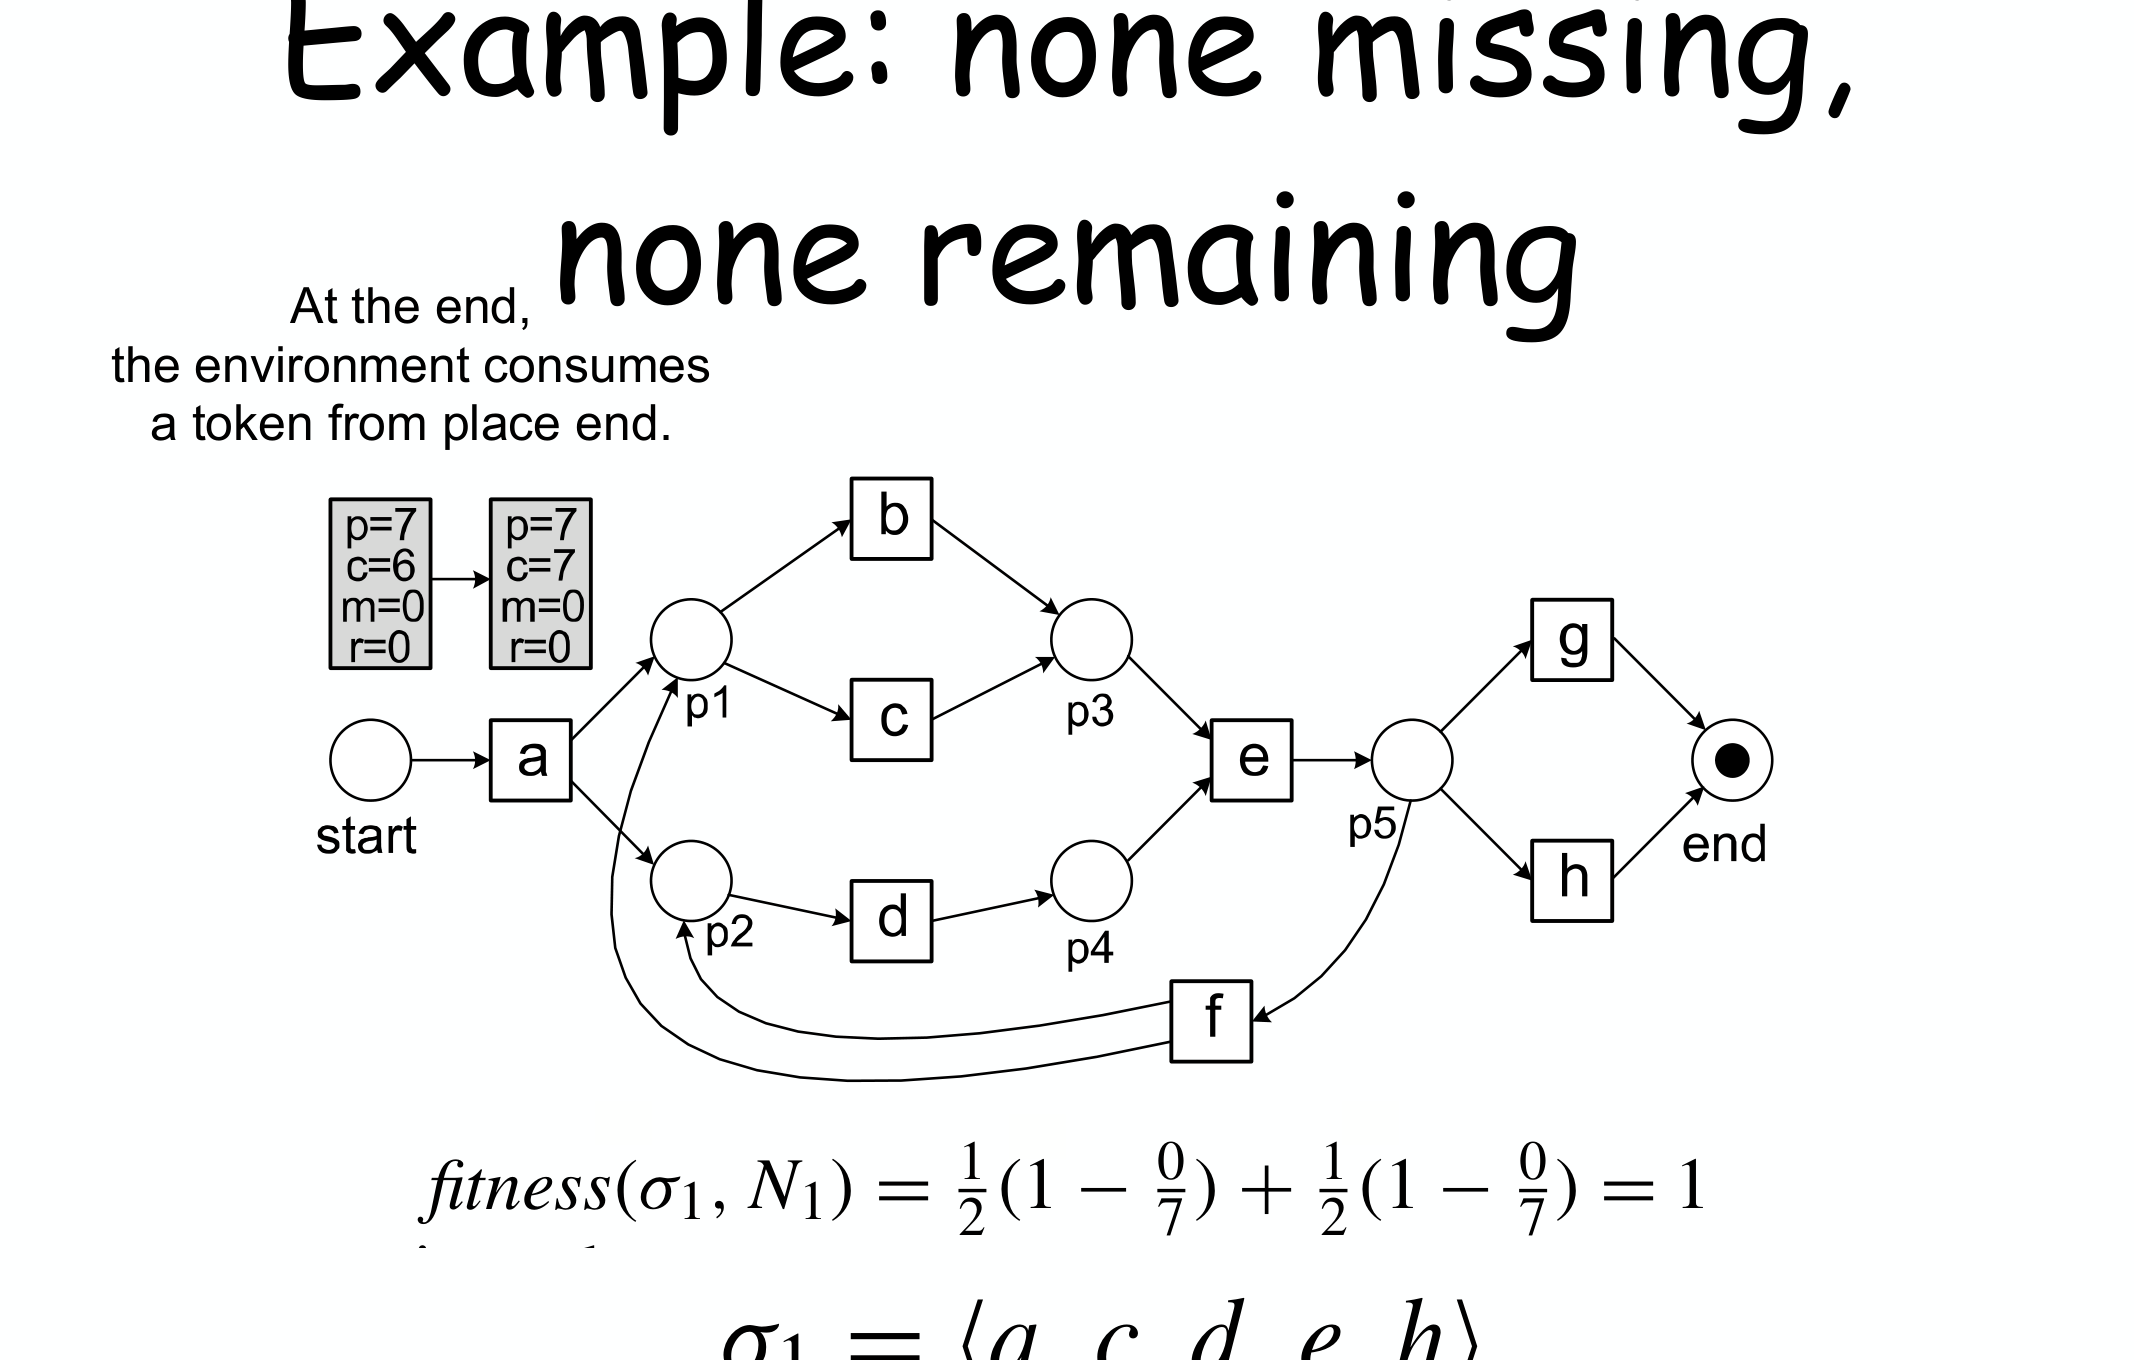
\includegraphics[width=0.74\linewidth,height=0.34\textheight,keepaspectratio]{images/19-conformance_p21_none-missing.png}
\caption{Riprodurre $\sigma_1 = \langle a,c,d,e,h\rangle$: ogni transizione trova sempre il token che le serve. Alla fine $m=r=0$ e $\text{fitness}(\sigma_1,N_1) = \frac12(1-0) + \frac12(1-0) = 1$: riproduzione perfetta.}
\end{figure}

\subsection{\texorpdfstring{Esempio: un token mancante}{Esempio: un token mancante}}

\begin{figure}[!htb]
\centering
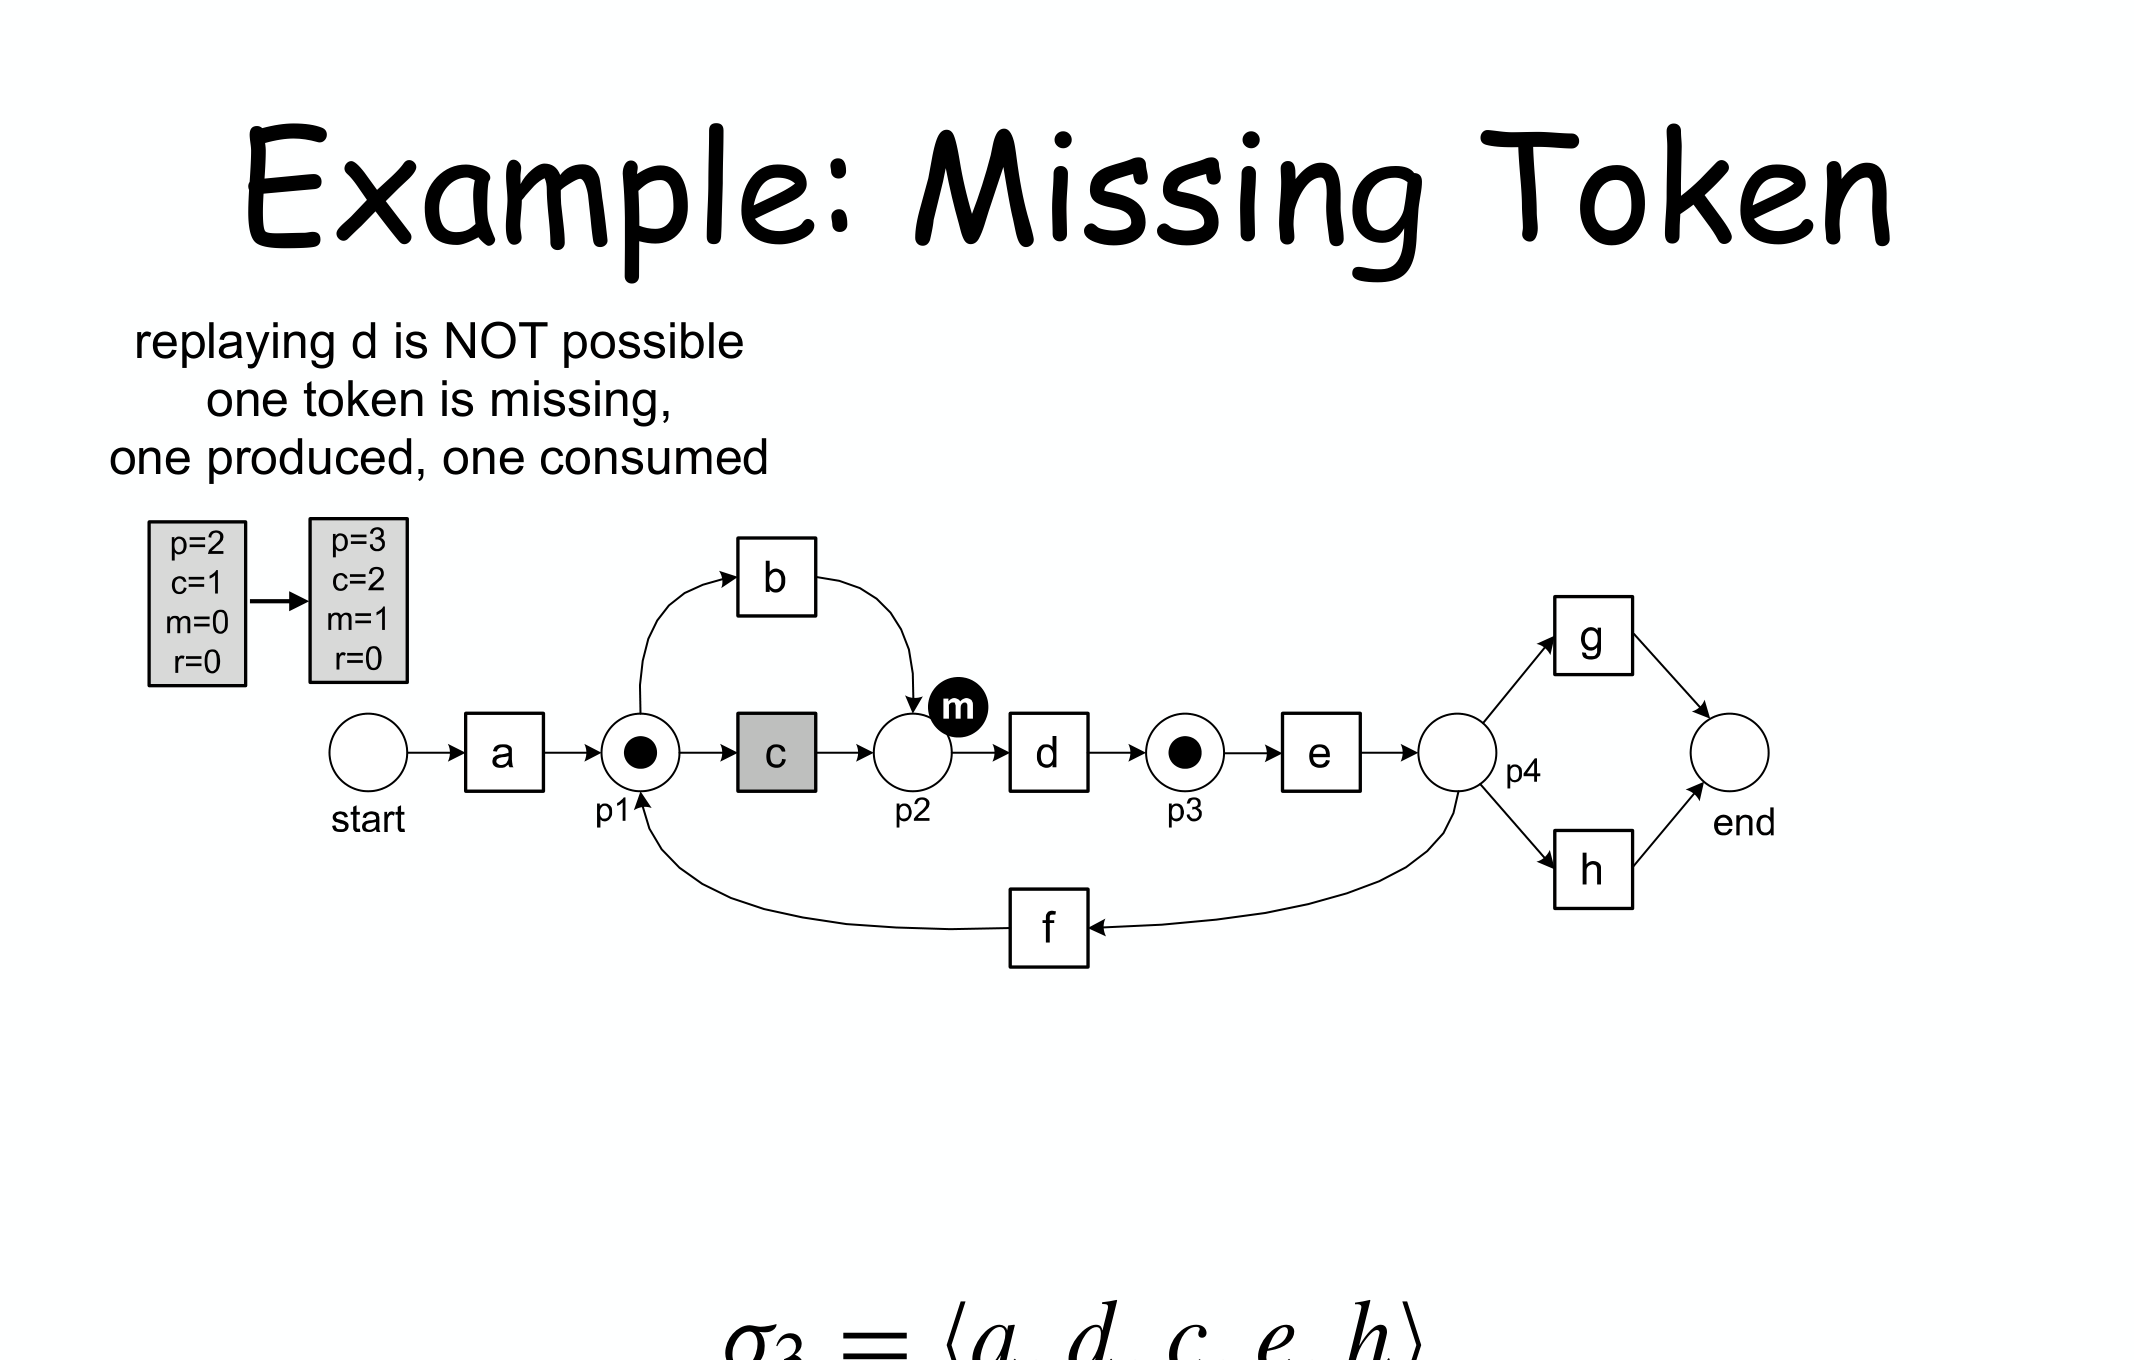
\includegraphics[width=0.74\linewidth,height=0.34\textheight,keepaspectratio]{images/19-conformance_p24_missing-token.png}
\caption{Riprodurre $\sigma_3 = \langle a,d,c,e,h\rangle$: qui l'ordine è invertito rispetto al modello (si tenta $d$ prima di $c$). $d$ ha bisogno del token che solo $c$ produce: \textbf{manca}, si forza comunque lo scatto (contatore $m$ aumenta di 1) e si prosegue. Fitness scende a $\frac12(1-\frac16)+\frac12(1-\frac16) = 0.833$: non conforme, ma "quasi" — molto più informativo del semplice non-fitting.}
\end{figure}

Un dettaglio tecnico da tenere a mente: se la trace contiene un evento che \textbf{non compare affatto} nel modello, quell'evento va semplicemente \textbf{rimosso} prima di riprodurla (non genera né token mancanti né residui — è solo "invisibile" al modello).

\subsection{\texorpdfstring{Dalla singola trace alla fitness dell'intero log}{Dalla singola trace alla fitness dell'intero log}}

La stessa formula si estende a un log completo sommando i contatori di tutte le trace, \textbf{pesate per la loro frequenza} (multiplicità) nel log:

\[
\text{fitness}(L,N) = \frac{1}{2}\left(1 - \frac{\sum_{\sigma \in L} L(\sigma) \cdot m_{N,\sigma}}{\sum_{\sigma \in L} L(\sigma) \cdot c_{N,\sigma}}\right) + \frac{1}{2}\left(1 - \frac{\sum_{\sigma \in L} L(\sigma) \cdot r_{N,\sigma}}{\sum_{\sigma \in L} L(\sigma) \cdot p_{N,\sigma}}\right)
\]

dove $L(\sigma)$ è quante volte la trace $\sigma$ compare nel log. Su questa base, i quattro modelli dell'esempio iniziale si separano finalmente in modo sensato:

\[
\text{fitness}(N_1) = 1
\]

\[
\text{fitness}(N_2) = 0.9504
\]

\[
\text{fitness}(N_3) = 0.8797
\]

\[
\text{fitness}(N_4) = 1
\]

Il flower model $N_4$ resta (giustamente) fuori discussione come "buon modello" per altri motivi (la sua precision è pessima), ma qui vediamo che la fitness da sola non basta a giudicare la qualità complessiva.

\section{\texorpdfstring{Diagnostica locale: dove sta il problema}{Diagnostica locale: dove sta il problema}}

Il token replay non dà solo un numero: annotando su \textbf{ogni place} quanti token sono mancati o rimasti, si ottiene una mappa visiva di \textbf{dove} il modello e la realtà divergono.

\begin{figure}[!htb]
\centering
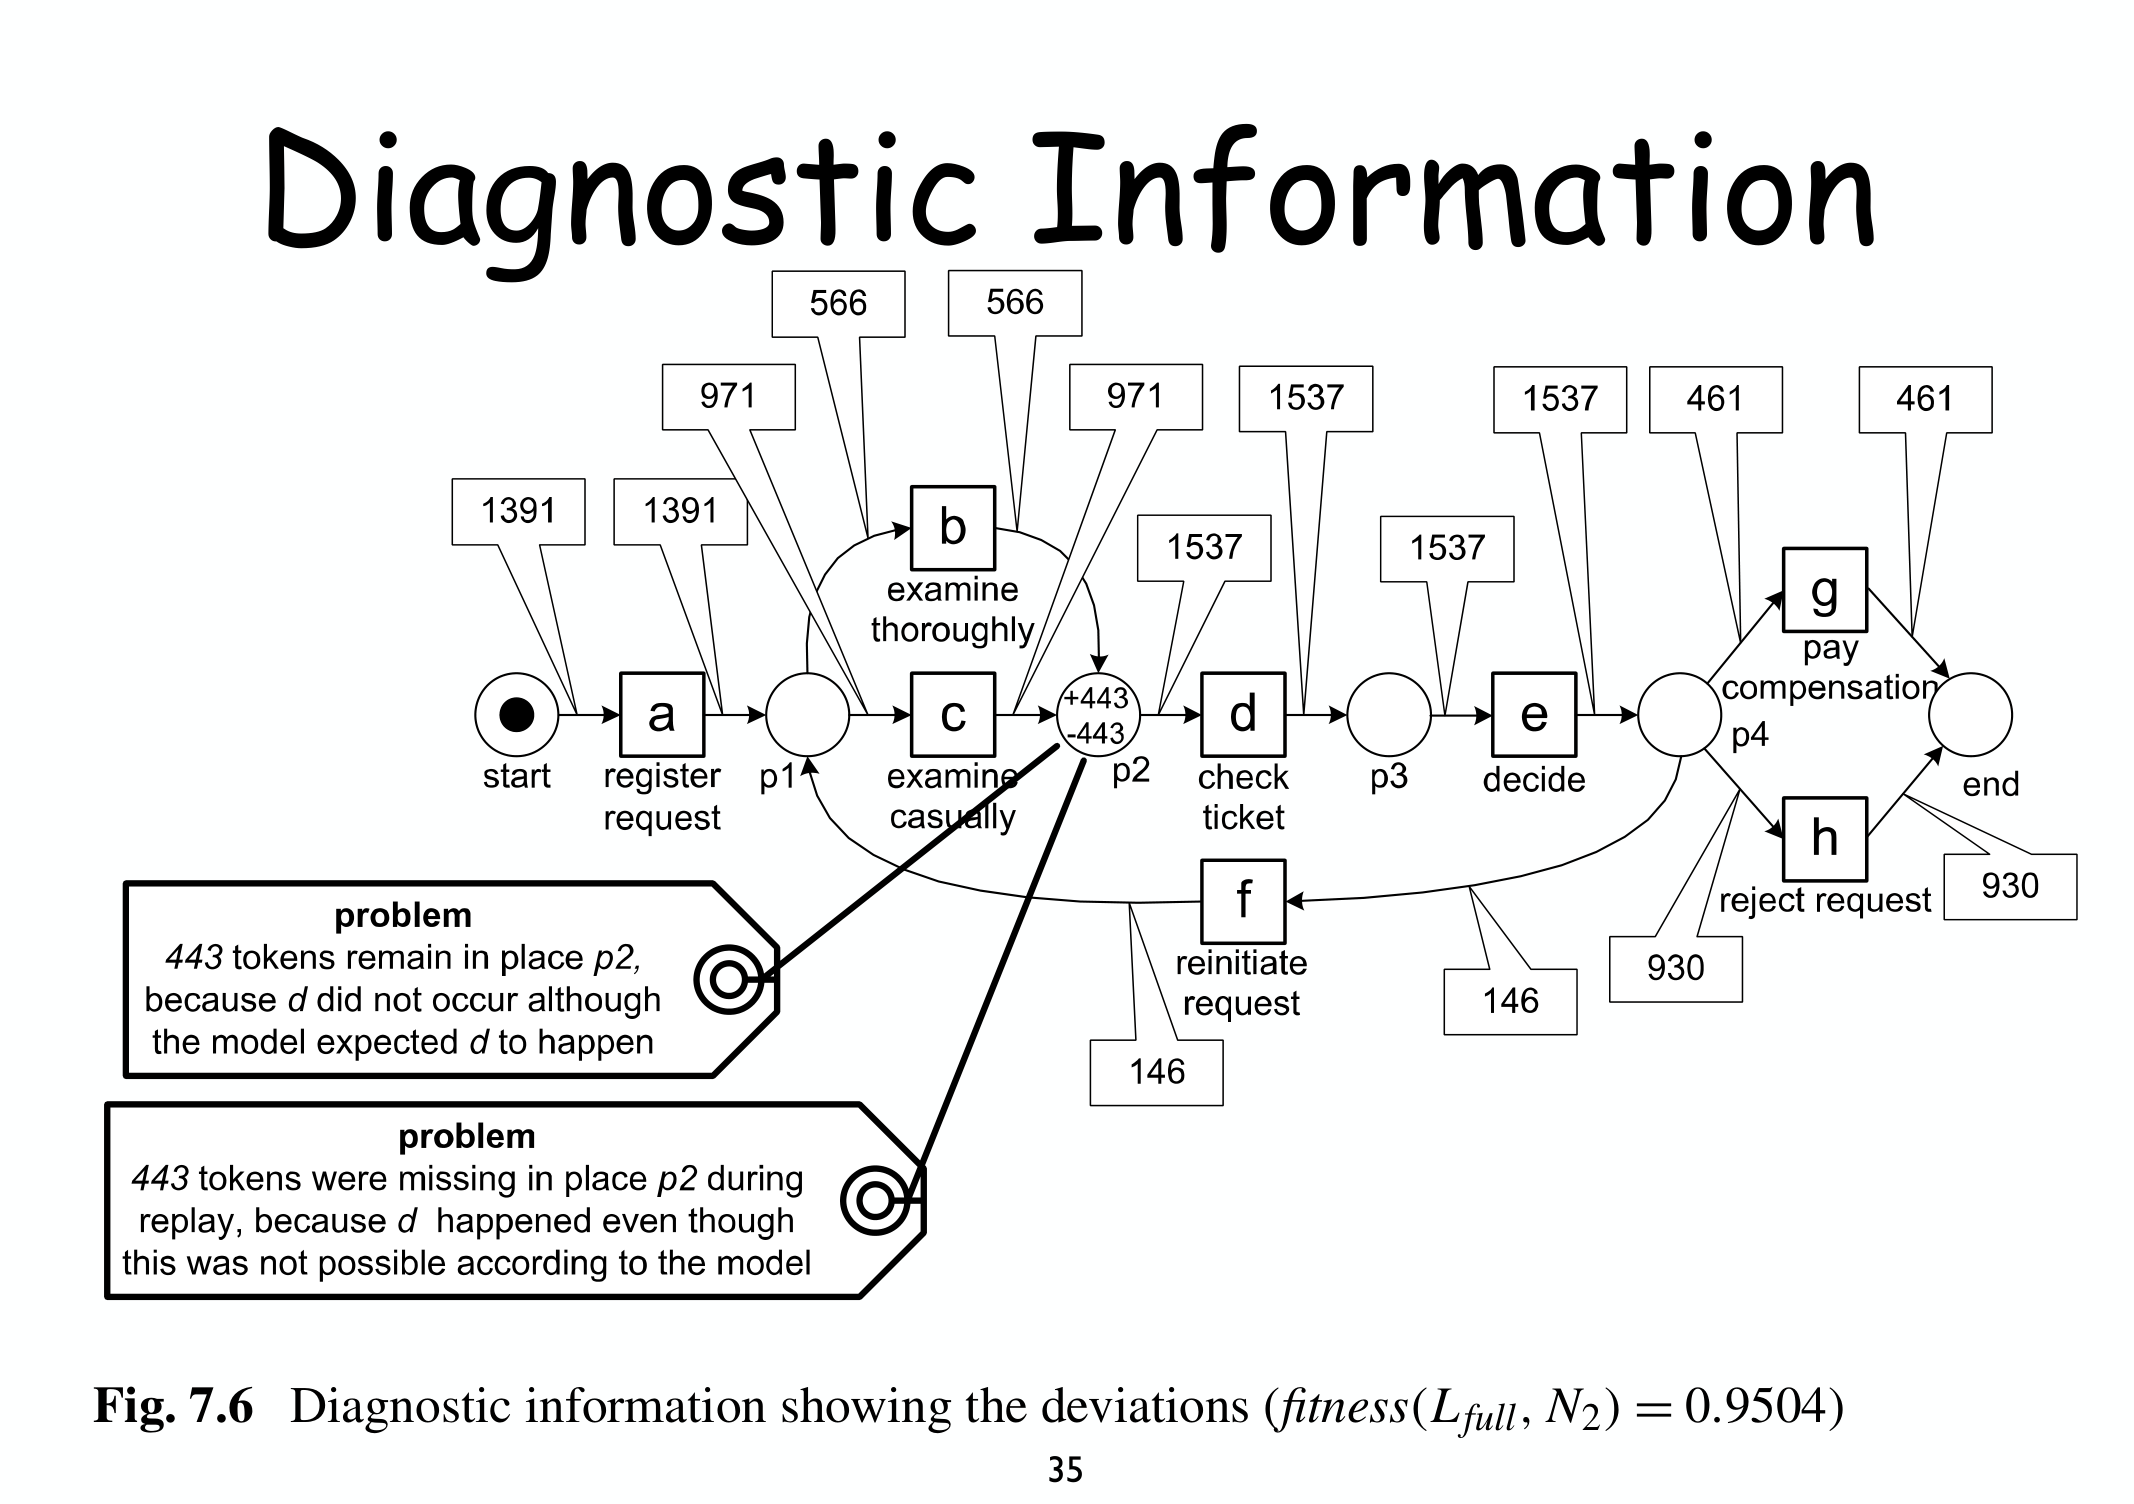
\includegraphics[width=0.74\linewidth,height=0.34\textheight,keepaspectratio]{images/19-conformance_p35_diagnostic-info.png}
\caption{Diagnostica su $N_2$ (fitness $=0.9504$): le etichette sugli archi mostrano quante volte ciascun percorso è stato realmente seguito; i due callout individuano \textbf{esattamente il place} ($p_2$) dove il modello si aspettava un ordine diverso da quello osservato. Non serve leggere l'intero log: il difetto è localizzato.}
\end{figure}

Questa diagnostica apre la porta a ulteriori analisi: si può \textbf{spezzare} il log in due sotto-log (i casi \emph{fitting} e quelli \emph{non-fitting}) e applicare tecniche diverse a ciascuno — ad esempio scoprire un modello \emph{separato} per i casi anomali, oppure incrociare i dati con altre informazioni (chi ha gestito i casi devianti, se sono costati di più, se richiedono più tempo — e nei casi di sospetta frode, persino costruire una rete sociale sui casi devianti).

\section{\texorpdfstring{Un'alternativa più leggera: i footprint}{Un'alternativa più leggera: i footprint}}

Il token replay richiede di eseguire davvero il modello, evento per evento. Un'alternativa più economica (e sufficiente per confronti rapidi) è basata sui \textbf{footprint} — la stessa matrice di relazioni causali vista nell'\hyperref[ch:05]{α-algorithm} ($\to$, $\leftarrow$, $\parallel$, $\#$), ma calcolata \textbf{sia dal log sia dal modello}, per poi confrontarle.

\begin{boxdefinition}{Footprint da un net (play-out)}
Dato un workflow net, la tecnica del \textbf{play-out} ne estrae un \textbf{insieme completo locale} di trace (cioè abbastanza trace da coprire ogni relazione di causalità presente nel modello). Trattando queste trace come un log (senza multiplicità), se ne deriva la stessa relazione $>$ dell'α-algorithm, e quindi il \textbf{footprint} del modello.

Un log si dice \textbf{completo} (rispetto al footprint) se ogni coppia di attività che \emph{può} susseguirsi lo fa \textbf{almeno una volta} nel log.
\end{boxdefinition}

Avere footprint sia per log sia per modelli apre a tre tipi di confronto:

\begin{boxnote}{Usi del confronto fra footprint}
\begin{itemize}
\item \textbf{log vs modello}: il log e il modello concordano?
\item \textbf{modello vs modello}: quantifica quanto due modelli si somigliano;
\item \textbf{log vs log}: rileva il \textbf{concept drift} — come cambia il modo di lavorare fra sotto-log diversi (es. prima e dopo una riorganizzazione)?
\end{itemize}
\end{boxnote}

La metrica di conformance basata sui footprint è semplicissima: si contano le celle \textbf{discordanti} fra le due matrici.

\begin{boxtheorem}{Conformance basata su footprint}
\(\text{conformance} = 1 - \frac{d}{n}\) dove $n$ è il numero totale di celle della matrice footprint e $d$ è il numero di celle nella \textbf{stessa posizione} ma con \textbf{contenuto diverso} fra le due matrici confrontate.
\end{boxtheorem}

\begin{figure}[!htb]
\centering
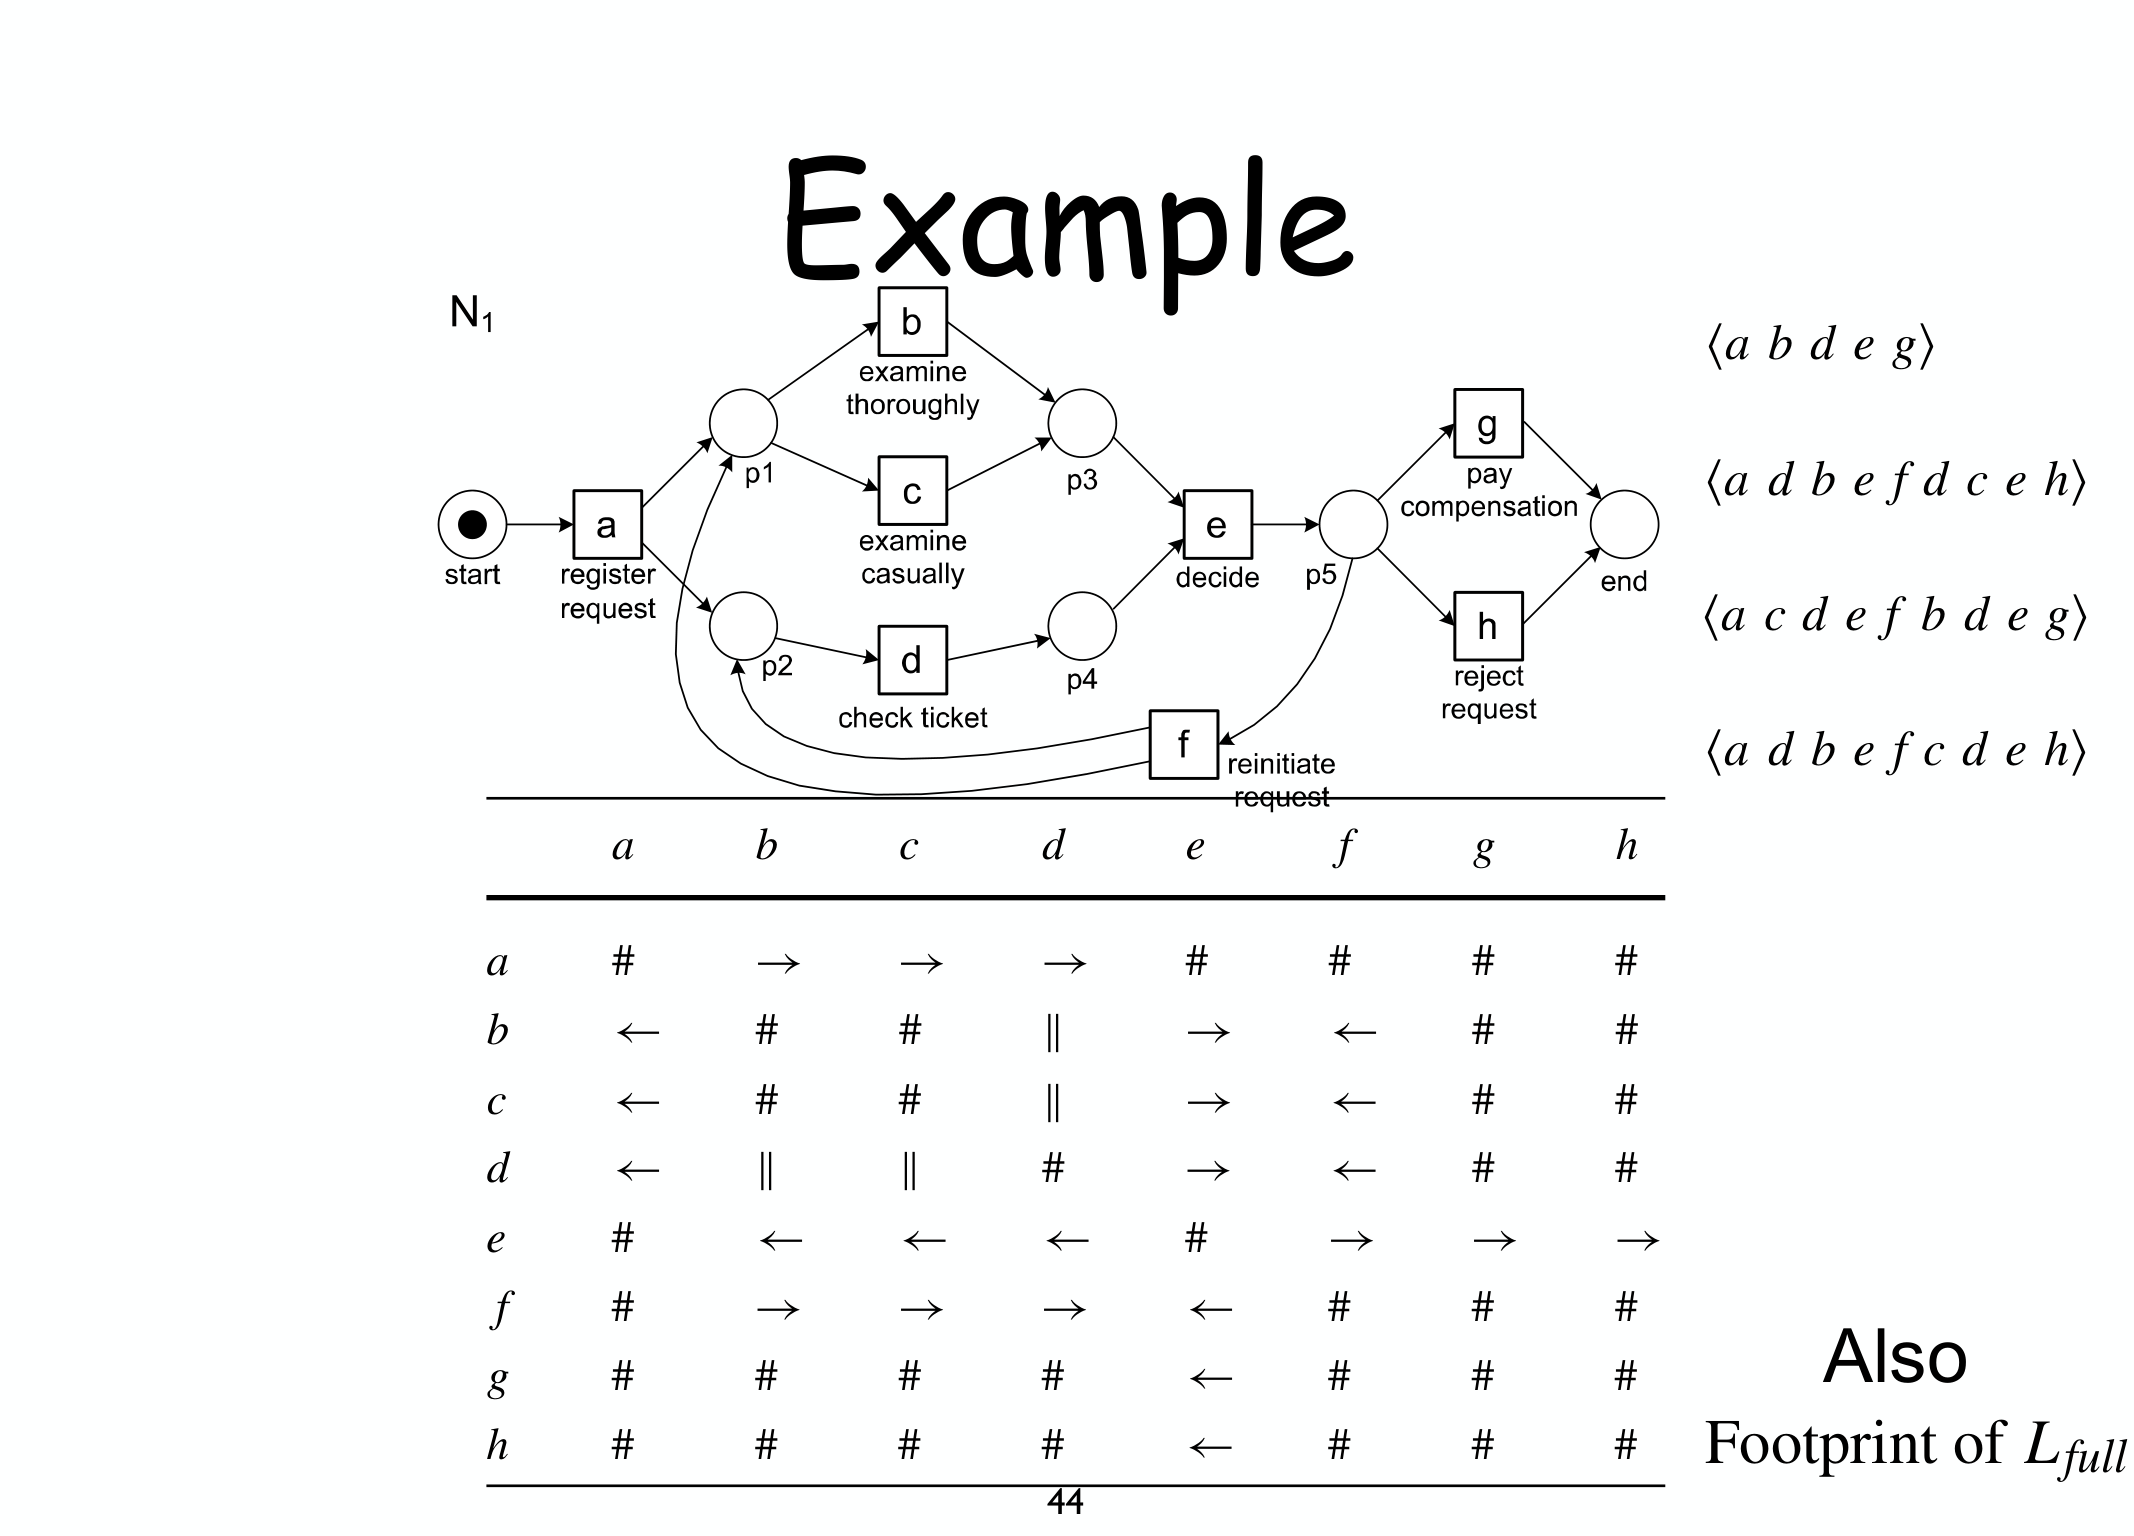
\includegraphics[width=0.74\linewidth,height=0.34\textheight,keepaspectratio]{images/19-conformance_p44_footprint-example.png}
\caption{Due footprint a confronto: \textbf{12 celle su 64} hanno un simbolo diverso (es. dove una matrice segna $\to$ e l'altra $\#$), dando conformance $1 - 12/64 = 0.8125$. Un calcolo puramente combinatorio, molto più leggero del token replay — ma anche più grossolano, perché non tiene conto delle frequenze reali delle trace.}
\end{figure}

\section{\texorpdfstring{Riepilogo}{Riepilogo}}

\begin{boxabstract}{Il quadro}
\begin{itemize}
\item La \textbf{fitness ingenua} (trace interamente riprodotta o scartata) è troppo grezza: non distingue "quasi conforme" da "completamente diverso".
\item Il \textbf{token replay} con i quattro contatori $p,c,m,r$ dà una fitness \textbf{granulare}, calcolabile per singola trace e aggregabile sull'intero log (pesata per frequenza).
\item La stessa riproduzione dà \textbf{diagnostica locale}: individua \emph{dove} nel modello nascono le discrepanze.
\item I \textbf{footprint} offrono un confronto più leggero (log vs modello, modello vs modello, log vs log), utile anche per rilevare il \textbf{concept drift}.
\end{itemize}
\end{boxabstract}

Con la conformance chiudiamo il ciclo completo del process mining: \textbf{discovery} (dai log al modello, \hyperref[ch:05]{05 — Process Mining}), \textbf{enhancement} (migliorare il modello) e ora \textbf{conformance} (verificare che modello e realtà coincidano). Le prossime lezioni tornano sull'analisi quantitativa e sulla diagnosi dei workflow net. $\rightarrow$ \hyperref[ch:20]{20 — Quantitative Analysis}